\section{Flow classification}
\label{section:rate:flow}

The aim of this section is to describe a process which distinguishes those flows which have their throughput limited by mechanisms other than the usual \ac{TCP} response to loss and delay.
Each flow can be characterized as being either application paced, in which the sending application is limiting the data provided, host limited, whereby local constraints at either end host cap throughput, or receiver shaped, in which an artificial constraint is imposed by either a middlebox or receiver.

One fundamental precondition to decouple the influence that network loss, host configuration and \ac{TCP} behaviour has on the throughput experienced by a flow is the reconstruction of the congestion window behaviour of \ac{TCP} flows on the basis of observed data. 
Unfortunately, the congestion window value is internal to the sender's \ac{TCP} state machine and may not manifest itself in the absence of sufficient data from the application layer. 
A more easily observed quantity which serves as a reasonable proxy for the congestion window is the number of unacknowledged bytes in flight, henceforth referred to as the \textit{flight size}, which can be derived given an accurate estimate of the end-to-end delay.
The evolution of both flight size and \ac{RTT} can in turn be used to ascertain to what extent throughput is regulated by limitations imposed at different layers of the networking stack.

% definitions
Given a stream of packets, the methodology presented in section \ref{section:malawi:rtt} can derive a candidate \ac{RTT} for a \ac{TCP} flow.
Given a candidate \ac{RTT}, a stream of packets with arrival times $t_1, t_2, \ldots$ can be aggregated into a stream of \emph{flights}. 
Intuitively, a flight is a clustered subset of a \ac{TCP} flow which exhibits its own temporal coherence; alternatively, it can be thought of as a series of consecutive packets that were (roughly) generated by the sender as a response to the same protocol operation. 
A flight $f_i$ that begins with the $j$th packet and ends with the $k$th is defined to have a \emph{total flight time} $\tau_i = t_{k+1} - t_j$. 
The algorithmic selection of initial and final packets in such a way that the resulting flights are indicative of \ac{TCP} behaviour remains an open problem. 
The \ac{RTT} is assumed to provide a natural time frame for the operation of \ac{TCP}.
As such, given an initial packet $\pi_j$ and an \ac{RTT} estimate $T$, the $k$th (and final) packet is selected to minimise \emph{the flight time error} $e_i = |T - \tau_i|$. 
This mechanism resembles the methodology described in \cite{Zhang:2002p85}, but where flights are not defined as being both adjacent and disjoint; rather, flows are decomposed into a stream of potentially overlapping flights. 
This helps the algorithm mitigate the deleterious effects of small deviations in the estimated \ac{RTT}, which alters the properties of each flight. 
Furthermore, since the flight size is continuous in time, it makes little sense to restrict window reconstruction to a single sample per round trip time.

Having obtained flight information from each flow, the predominant factor that affects its throughput can be determined.
Within the context of \ac{TCP}, flows are classified as being artificially constrained by three distinct processes: \emph{application pacing}, \emph{host limited} and \emph{receiver shaping}.


\subsection{Application paced}
\label{section:rate:app}

\begin{figure}
\centering
  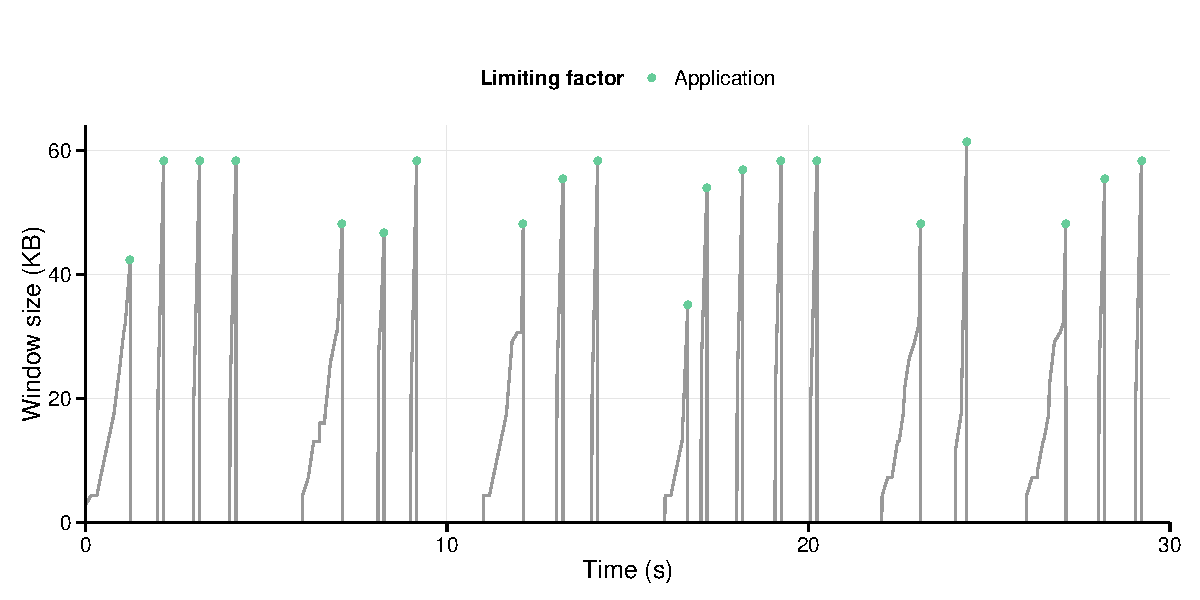
\includegraphics[width=0.8\textwidth]{figures/malawi/youtube.pdf}
  \caption{Congestion window over time for application paced flow. \label{fig:youtube}}
\end{figure}

A flow whose throughput decreases because it has no outstanding data to send is temporarily limited by the application. 
Flights can be identified as being \emph{application limited} if terminated with a packet smaller than the \ac{MSS} and followed by an inter-arrival time greater than the \ac{RTT}, as consistent with \cite{Zhang:2002p85}. 
The underlying reason for this defintion is that most \ac{TCP} implementations will wait some time for subsequent bytes to be written to the socket if the next packet to be sent is smaller than the \ac{MSS}, unless the \ac{TCP}\_NODELAY option is set \cite{Nagle:1984p458}.

A flow with \emph{application limited} flights however is not necessarily \emph{application paced}. 
In practice, all flows for which the final packet is observed contain at least one such flight.
For the purposes of this work however, the focus remains on identifying cases in which throughput is predominantly determined by application behaviour.
One such example is illustrated in figure \ref{fig:youtube}, in which a stream is delivered by periodically writing blocks to the sending socket.
The resulting network-level behaviour is distinct from traditional congestion control: short bursts are interspersed with protracted silence.
Application limited flights, which terminate on non-\ac{MSS} packets, are highlighted at the end of each burst.

This behaviour is in stark contrast to that exhibited in figure \ref{fig:hostlimited}, where distinct transfers are multiplexed on top of a single transport association over time.
From the perspective of the network, there is little to distinguish the behaviour of such traffic from independent \ac{TCP} flows.
Application paced connections such as Youtube traffic however exhibit a degree of regularity which can potentially be exploited by the network in predicting demand or smoothing bursts.

In order to identify such recurring behaviour, flows are classified as being \emph{application paced} if the period between bursts terminated by \emph{application limited flights} is consistently under 10 seconds and the standard deviation of the intermediate pauses is under one second.
This definition in particular purposely ignores flows which exhibit long silence periods due to user interaction, and follows closely the behaviour historically associated to Youtube streaming in particular.

\subsection{Host limited}
\label{section:rate:host}

Given sufficient bandwidth and traffic to send, a flow may encounter local constraints at either end-host which caps its throughput. 
For instance, the buffer space allocated on both the sender and receiver side is often pre-configured, and it is common practice to tune these values down on popular servers and managed infrastructure in a bid to conserve memory or bandwidth.
A receiver is also limited in the window size it can announce to the remote sender; if the windowscale option \cite{jacobson1992tcp} is not negotiated during the \ac{TCP} handshake, the advertised window cannot exceed 64KB.

\begin{figure}
\centering
  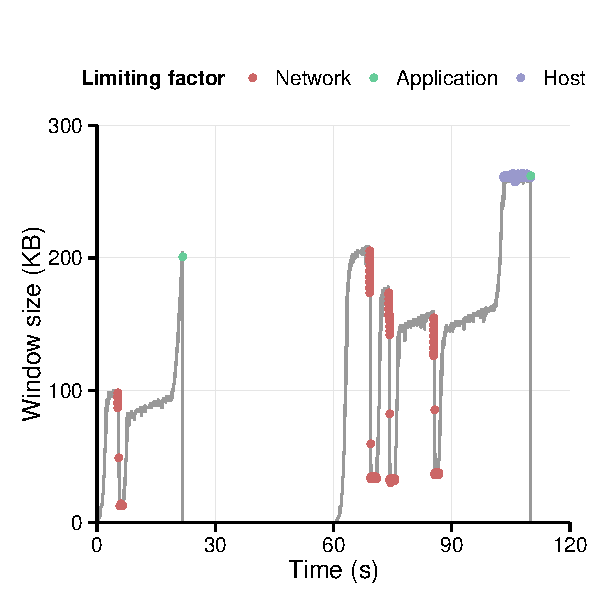
\includegraphics[width=0.8\textwidth]{figures/malawi/hostflow.pdf}
  \caption{Congestion window over time for partially host limited flow. \label{fig:hostlimited}}
\end{figure}

In both cases, a local decision by either host can determine the upper bound of the flow rate.
These \emph{host limited} cases are characterised by a constant window size over time.
The methodology described for flight aggregation at the beginning of this section typically generates a large number of flights, representing many likely combinations given a base \ac{RTT} estimate.
In order to identify the flat-lined behaviour of a host limited flow, the flight stream is first filtered to remove some of the uncertainty derived from small fluctuations in the \ac{RTT}.
The maximum flight size observed for each \ac{RTT} interval is then selected, with a sequence of flights being classified as host limited if the same maximum was observed over six consecutive \acp{RTT} (this is twice the period suggested in \cite{Zhang:2002p85}).
In practice, increasing the period over which the maximum window size is tracked allows us to more accurately discern between host limited behaviour and more conservative bandwidth probing, such as that performed during the convex phase of \ac{TCP} CUBIC \cite{Ha:2008p471}.

A flow may be host limited for only brief periods of its lifetime, as illustrated in figure \ref{fig:hostlimited}.
To filter out such cases where host limitations are not the predominant factor in defining flow throughput, a further requirement is imposed for a flow to be classified as being host limited: the average window size over a flow lifetime should be within 10\% of the inferred host limit, which is not the case in figure \ref{fig:hostlimited}.
In practice, flows can exhibit both application pacing and host limitations, with bursts being sent at a capped window size followed by application pauses.
In such cases, a flow will still be classified as being \emph{application paced} if it meets the requirements set out in the previous section, as doing so provides evidence that it controls throughput in spite of the degraded performance provided further down the stack. 
This line of reasoning applies equally to the occurrence of sporadic loss; so long as block delivery is ensured within the time frame dictated by the application, it remains in control.

\subsection{Receiver shaped}
\label{section:rate:recv}

A flow which is neither \emph{application paced} or \emph{host limited} can still be artificially constrained by flow control (rather than by congestion control).
Traditionally, in \ac{TCP} the sender is responsible for regulating throughput. 
However, the receiver can also shape throughput by manipulating the \emph{advertised window} announced on every acknowledgement.
Such receiver window auto-tuning has been available on Windows operating systems since Vista \cite{vistaReceiveWindow}, and can also be leveraged by middleboxes to throttle inbound traffic \cite{appEx}.
To evaluate the potential impact of such behaviour, a further heuristic is proposed to identify receiver-shaped traffic.
For flows in which both directions of traffic are observed it is possible to correlate the evolution of the advertised window with the size of reconstructed flights.
Figure \ref{fig:awnd} displays an example of a receiver-shaped connection, in this case throttled by an intermediate middlebox.
Since the advertised window may be fluctuating, it is not always obvious which of the many updates were effectively applied by the sender as successive values supersede each other.
An example of a reconstructed flow which is subjected to receiver shaping is displayed in Figure \ref{fig:awnd}.

\begin{figure}
\centering
  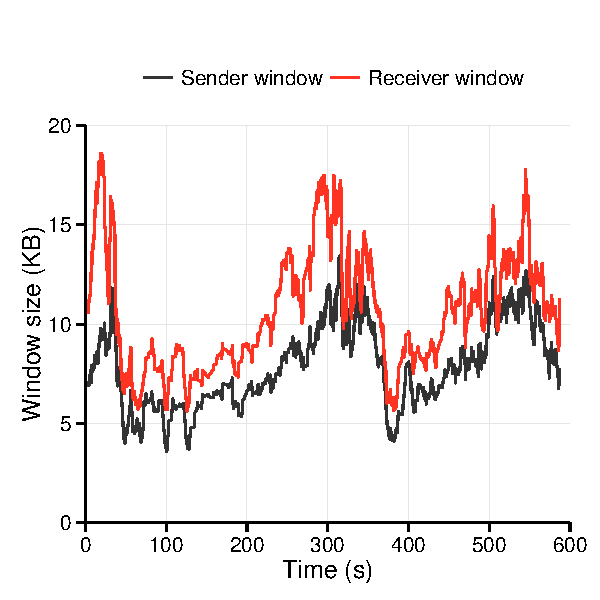
\includegraphics[width=0.8\textwidth]{figures/malawi/awnd.pdf}
  \caption{Congestion window over time for receiver limited flow. \label{fig:awnd}}
\end{figure}

For flows in which both directions are observed, it is possible to classify flights as being receiver-shaped if there is a statistically significant correlation between the advertised window size and the maximum flight size observed.
Harnessing the stream filtering used in detecting host limited behaviour, such analysis is performed over a sliding window of 10 \ac{RTT} intervals.
A flight is flagged as being receiver shaped if the correlation between receiver window and flight size is statistically significant; a flow is considered to be predominantly receiver shaped if over half of its flights are flagged as such.
This covariance analysis is not performed on flights which contain out-of-order or retransmitted packets. 
In such cases both the receiver and sender window sizes are correlated \emph{by definition}: the receiver buffer will temporarily fill expecting the next packet in sequence while the sender will reduce its congestion window due to temporary setback in \ac{ACK} clocking.

Given that receiver shaping classification requires correlating information in both directions of a \ac{TCP} connection, it will come as no surprise that the absence of the reverse path can introduce false positives into our measurements. 
This happens because any given flow might be receiver shaped in such a manner that the heuristic erroneously attributes its behaviour to host limitations. 
In the absence of additional evidence, this misclassification is difficult to detect explicitly. 
Instead, the ratio of receiver shaped flows which would have been incorrectly identified is calculated for cases where the reverse path was not observed. 
This error rate can then be used to evaluate the accuracy of classifier results.
